\subsection{Student states with dense teacher feedback}

Offline distillation is dense but trains only on teacher-generated prefixes, so an early
student error can enter an unseen state. Outcome-reward RL samples student states, but its
terminal score does not localize the mistake. OPD retains the student trajectory and asks
the teacher to score every sampled token under its exact student-generated prefix.

The teacher does not replace the rollout. It asks how plausible the next token was given
the student's exact prefix. Figure~\ref{fig:opd-token-feedback} shows an early redirecting
token receiving a strong penalty while the now-predictable final error receives little.

\begin{figure}[htbp]
  \centering
  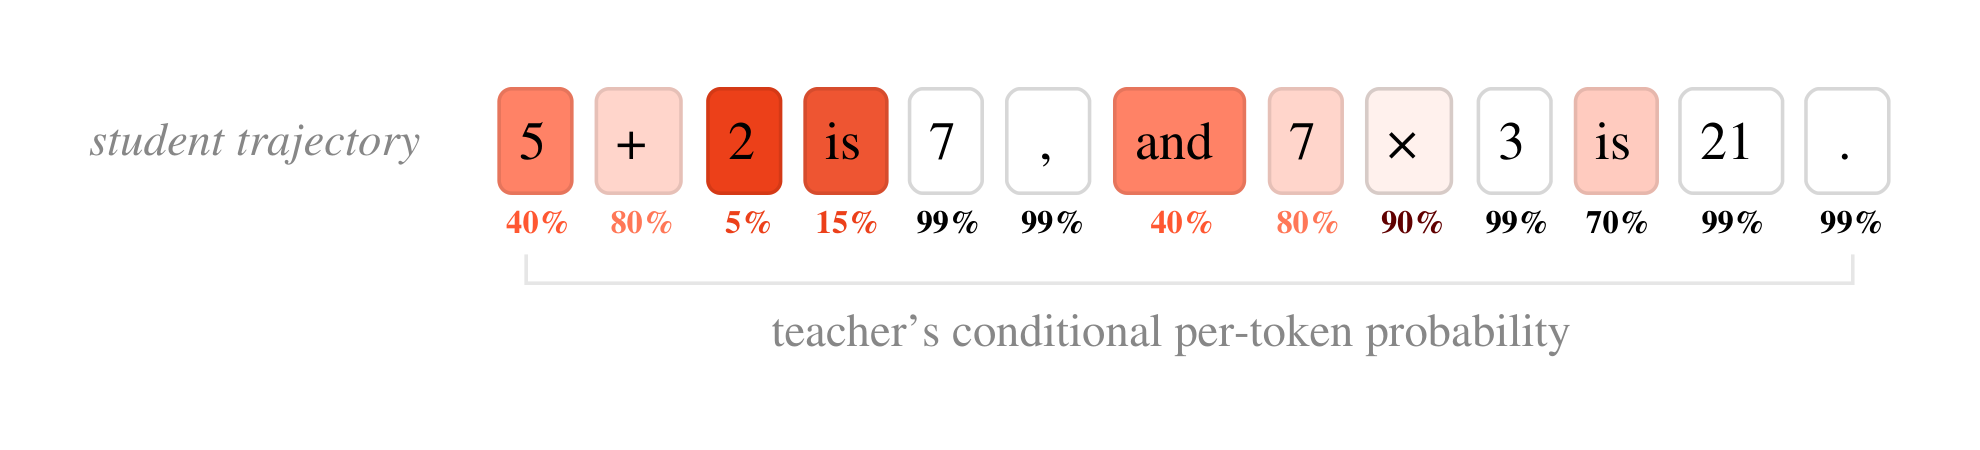
\includegraphics[width=0.88\textwidth]{figures/thinking_machines_opd_token_feedback.png}
  \caption{Teacher probabilities for each token in a student trajectory; darker red means
  lower probability under the exact student prefix. Reproduced from Thinking Machines
  Lab \citep{lu2025onpolicydistillation}.}
  \label{fig:opd-token-feedback}
\end{figure}
